\section{Boundary conditions}%
\label{sec:boundary_conditions}
A number of different boundary conditions can be used for various modeling goals. Below we list the ones that are used in this paper. We select, for each of the four boundaries $\Gamma_d$ of $\Omega$, one of the conditions listed below. All conditions (except for the inflow condition in Section~\ref{sec:continuous_inflow}) are built to either dissipate or conserve kinetic energy. More precisely, we choose to impose boundary conditions at $\Gamma_d$ which lead to
\begin{equation}
  \label{eq:energy_gamma_d}
  -\ipbcpart{\wcn}{|\wc|^2} - 2\ipbcpart{\wcn}{p} \leq 0 \,.
\end{equation}
Note that
\begin{equation*}
  \ipbc{\wcn}{|\wc|^2} + 2\ipbc{\wcn}{p} = \sum_d \left(\ipbcpart{\wcn}{|\wc|^2} + 2\ipbcpart{\wcn}{p} \right) \,.
\end{equation*}
Hence, if~\eqref{eq:energy_gamma_d} is satisfied for all four boundaries, Proposition~\ref{prop:kinetic_energy_bound} implies that the kinetic energy does not grow.

As we shall see in Section~\ref{sec:discrete_boundary_conditions}, the continuous bounds are mimicked in the discrete setting by using encapsulated SBP operators and weakly imposed boundary conditions.

\subsection{Solid wall}
To model a solid wall we may impose vanishing normal velocity, $\wcn = 0$, so that the boundary terms in~\eqref{eq:energy_gamma_d} cancel. Figure~\ref{fig:cavity_flow} shows a simulation of a cavity flow using this boundary condition on the entire boundary $\partial \Omega$.
\begin{figure}%
  \centering
  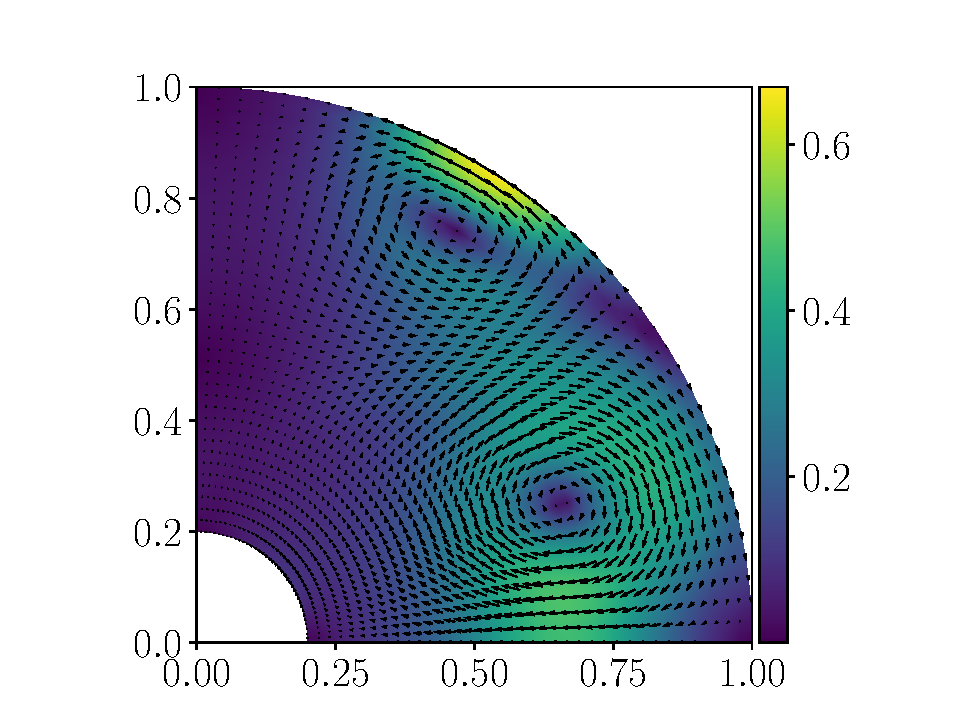
\includegraphics[width=0.7\textwidth]{images/cavity_flow.pdf}
  \caption{Flow inside an annulus sector with the boundary condition $\wcn = 0$ imposed on all four boundaries.}%
  \label{fig:cavity_flow}
\end{figure}

\subsection{Pressure outflow}\label{sec:pressure_outflow}
If $\wcn > 0$  on $\Gamma_d$ it suffices to specify the pressure $p$. Indeed, if $\wcn > 0$ and a nonnegative pressure $p$ is imposed, then $-\ipbcpart{\wcn}{|\wc|^2} - 2\ipbcpart{\wcn}{p} \leq 0$. This can be used to model a priori known outflow boundaries, for example a horizontal flow inside a channel (see Figure~\ref{fig:bump_flow}).

\subsection{Stabilized pressure outflow}%
\label{sub:stab_pressure}
Only prescribing the pressure as described in Section~\ref{sec:pressure_outflow} will lead to instability if the boundary changes from an outflow to an inflow, since $-\ipgd{\wcn}{|\wc|^2} - 2\ipgd{\wcn}{p} > 0$ if $\wcn < 0$. Consider instead the boundary condition
\begin{equation}
  \begin{aligned}
    h(\wcn) \wcn^2 + 2p & = 0
    \\
    h(\wcn) \wct^2 & = 0
  \end{aligned}
  \quad \quad \text{where} \quad
  h(\wcn) =
  \begin{cases}
     1 \quad \text{if} \quad \wcn < 0
     \\
     0 \quad \text{if} \quad \wcn \ge 0
  \end{cases}
  \,.
  \label{eq:stabilized_outflow}
\end{equation}
Here, $\wct = -n_y u + n_x v$ is the tangential velocity. If $\wcn \geq 0$, then~\eqref{eq:stabilized_outflow} is reduced to the pressure outflow condition. If $\wcn < 0$, then the condition $\wcn^2 + p = 0$ serves to attract the fluid since it decreases the pressure at the boundary, while the condition $\wct = 0$ restricts tangential flow (see Figure~\ref{fig:stab_pressure}). Furthermore, if $\wcn < 0$, imposing~\eqref{eq:stabilized_outflow} on $\Gamma_d$ yields
\begin{equation*}
  -\ipbcpart{\wcn}{|\wc|^2} - 2\ipbcpart{\wcn}{p} = -\ipbcpart{\wcn}{\wcn^2 + \wct^2 + 2p} = 0 \,.
\end{equation*}

\begin{figure}%
  \centering
  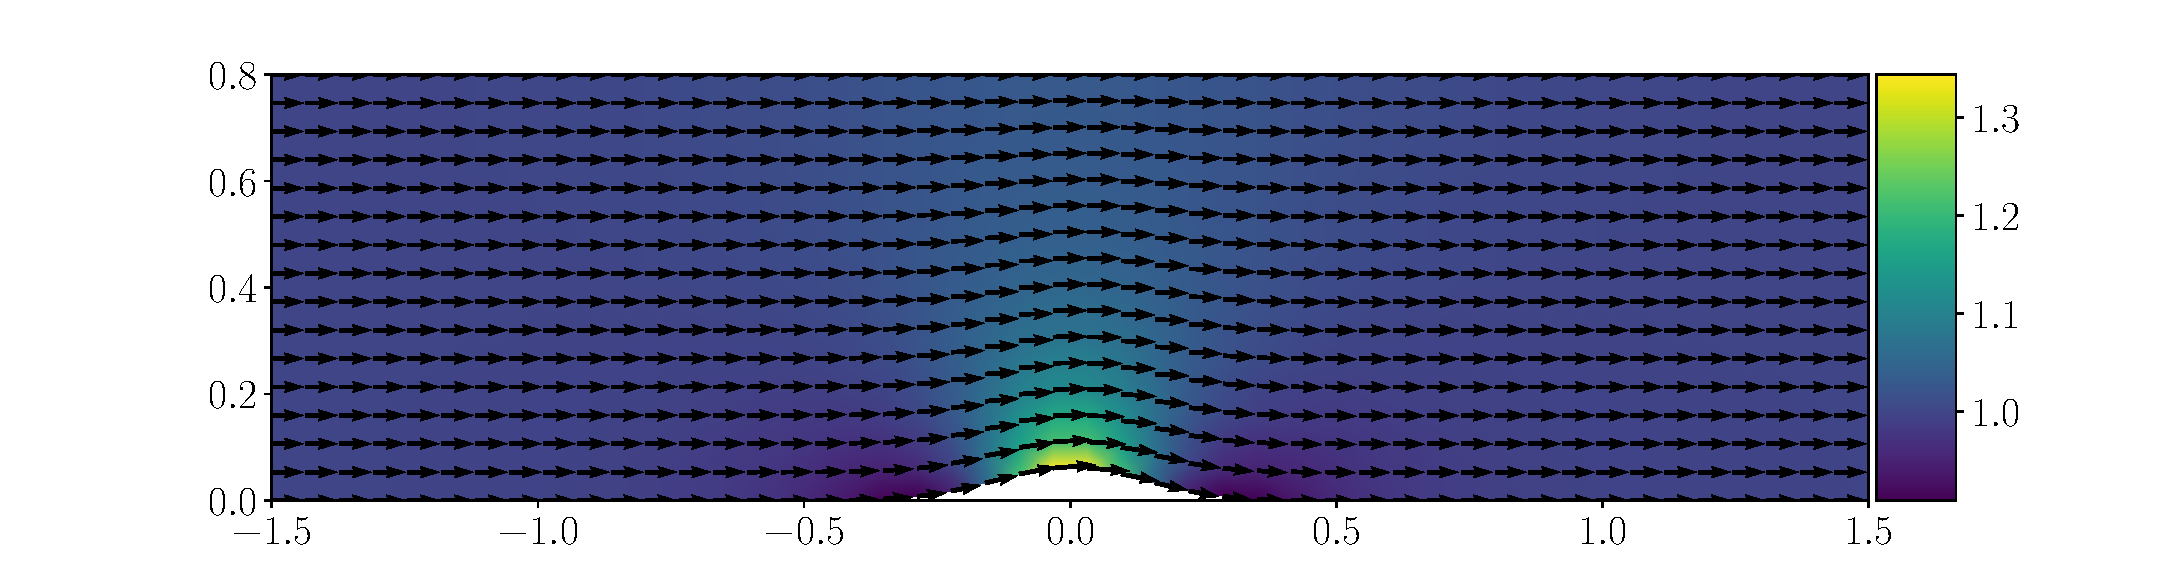
\includegraphics[width=\textwidth]{images/bump_flow.pdf}
  \caption{Flow inside a channel with a bump.}%
  \label{fig:bump_flow}
\end{figure}

\subsection{Inflow}\label{sec:continuous_inflow}
To model an inflow boundary we may impose the conditions $\wcn = g_n$ and $\wct = g_s$, specifying the normal and tangential velocity. Note that this implies that
\begin{equation*}
  -\ipbcpart{\wcn}{|\wc|^2} - 2\ipbcpart{\wcn}{p} = -\ipbcpart{g_n}{g_n^2 + g_s^2} - 2\ipbcpart{g_n}{p} \,,
\end{equation*}
which is only bounded in terms of data under the assumption that $p$ is bounded. To the best of our knowledge, there is no proof that $p$ is bounded. Our numerical experiments do not exhibit any issues related to uncontrolled growth in $p$, but the inflow boundary condition should still be used with care since there is no formal guarantee that the kinetic energy will not grow unexpectedly.
\begin{figure}%
  \centering
  \begin{subfigure}{0.24\textwidth}
    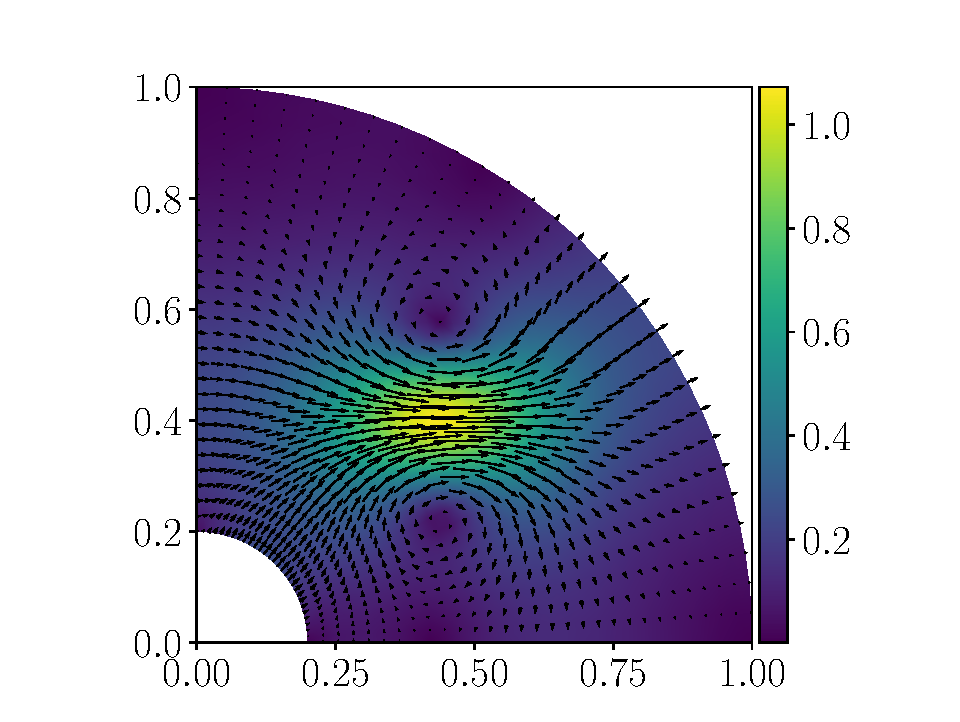
\includegraphics[width=\textwidth]{images/outflow1.pdf}
  \end{subfigure}
  \begin{subfigure}{0.24\textwidth}
    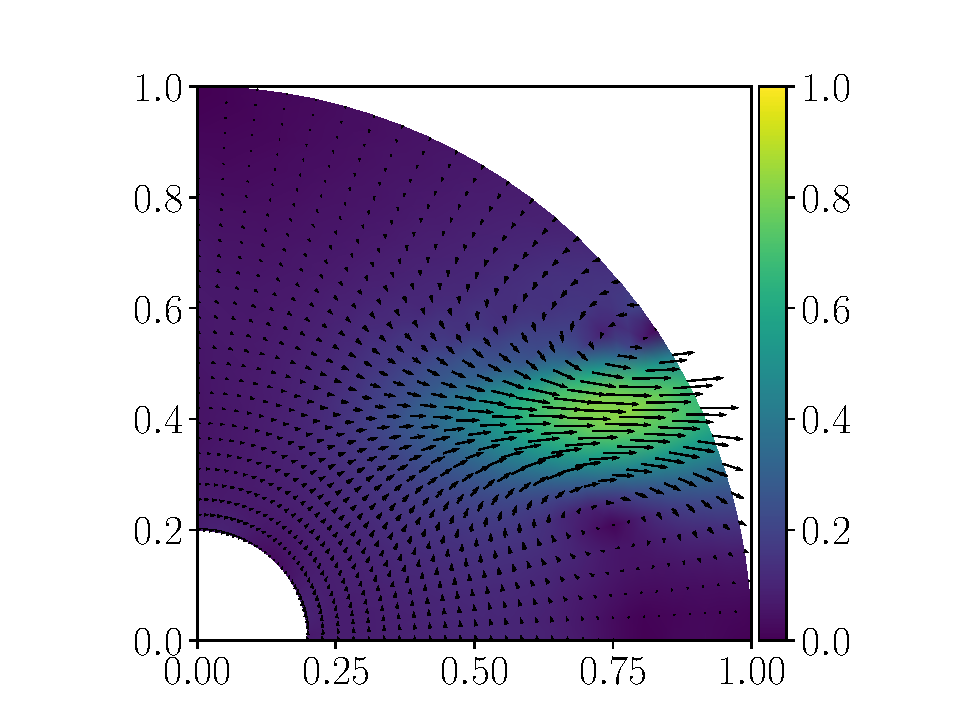
\includegraphics[width=\textwidth]{images/outflow2.pdf}
  \end{subfigure}
  \begin{subfigure}{0.24\textwidth}
    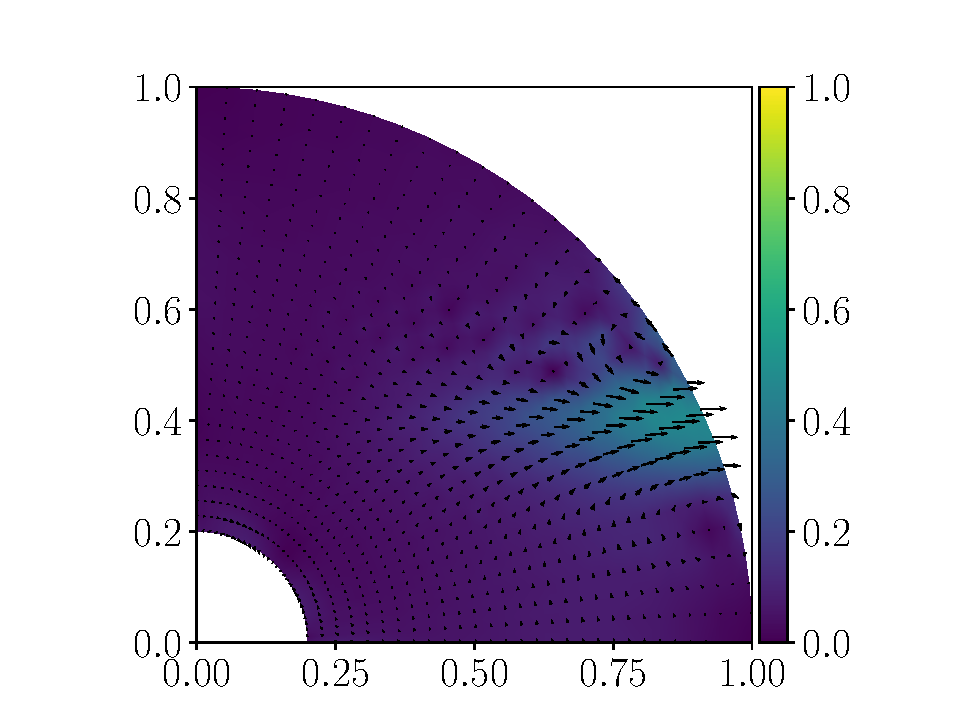
\includegraphics[width=\textwidth]{images/outflow3.pdf}
  \end{subfigure}
  \begin{subfigure}{0.24\textwidth}
    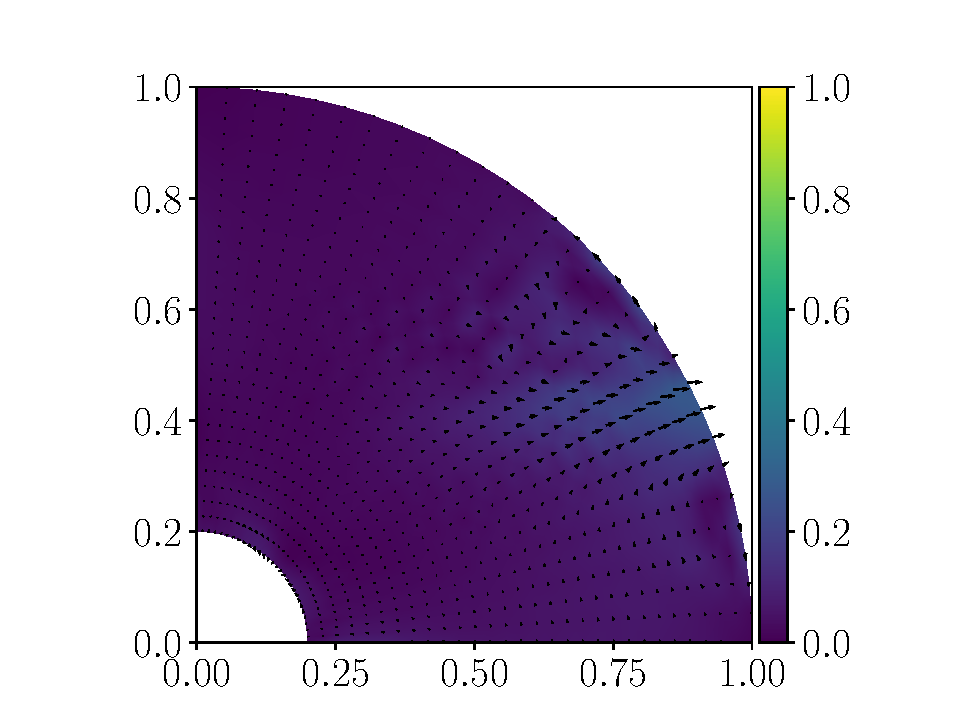
\includegraphics[width=\textwidth]{images/outflow4.pdf}
  \end{subfigure}
  \caption{A simulation initialized with $\vn = \pn = \zeron$, and a Gaussian bell in $\un$, resulting in swirling fluid exiting the domain through a boundary using the stabilized pressure condition.}%
  \label{fig:stab_pressure}
\end{figure}
